\documentclass[final,5p,times,twocolumn]{elsarticle}

\usepackage{lineno,hyperref}
\modulolinenumbers[5]

\usepackage{booktabs} % For formal tables
\usepackage{graphicx}
\usepackage{float}
\usepackage{listings}
\usepackage{xcolor}
\usepackage{geometry}
\usepackage{tikz}
\usetikzlibrary{shapes,arrows,positioning}
\usepackage{caption}
\usepackage{subcaption}

\journal{SoftwareX}

%% Elsevier bibliography styles
\bibliographystyle{elsarticle-num}

\begin{document}

\begin{frontmatter}

\title{ResearchShop Disease2Gene: A Validated Automated Pipeline for Gene-Disease Association Extraction from Full-Text Biomedical Literature}

%% Group authors per affiliation:
\author{Michał Bujniewicz-Uppal\corref{mycorrespondingauthor}}
\address{Interdisciplinary Centre for Mathematical and Computational Modelling, University of Warsaw, Warsaw, Poland}
\cortext[mycorrespondingauthor]{Corresponding author}

\author{Catherine Suski-Grabowski}
\address{Interdisciplinary Centre for Mathematical and Computational Modelling, University of Warsaw, Warsaw, Poland}

\author{Łukasz Górski}
\address{Interdisciplinary Centre for Mathematical and Computational Modelling, University of Warsaw, Warsaw, Poland}

\begin{abstract}
The exponential growth of biomedical literature necessitates automated tools to extract gene-disease associations. However, existing Large Language Model (LLM) approaches often suffer from "hallucinations," generating plausible but incorrect associations. We present ResearchShop Disease2Gene, a comprehensive software pipeline that automates the extraction of these associations from full-text literature. Uniquely, it integrates a multi-layer validation framework that verifies gene symbols against the HUGO Gene Nomenclature Committee (HGNC) database, validates genomic variants using HGVS standards, and performs citation cross-referencing to ensure extracted evidence exists in the source text. This software enables researchers to reliably mine vast literature repositories for high-confidence genetic evidence, bridging the gap between publication volume and actionable clinical insights.
\end{abstract}

\begin{keyword}
Gene-disease association \sep Biomedical text mining \sep Large Language Models \sep Hallucination mitigation \sep Full-text processing
\end{keyword}

\end{frontmatter}

% \linenumbers

\section*{Current Code Version}
\label{sec:metadata}
\noindent\textbf{Metadata}\par
\vspace{0.45em}
{\footnotesize
\setlength{\tabcolsep}{5pt}
\renewcommand{\arraystretch}{1.05}
\begin{tabularx}{\textwidth}{>{\raggedright\arraybackslash}p{0.7cm} >{\raggedright\arraybackslash}p{4.0cm} X}
\toprule
\textbf{Nr.} & \textbf{Code metadata description} & \textbf{Metadata} \\
\midrule
C1 & Current code version & v1.0.1 \\
C2 & Code/repository link & \url{https://github.com/michaluppal/Researchshop-Disease2Gene} \\
C3 & Compute environment & Local desktop (Electron + Python virtual environment) \\
C4 & Legal code license & Apache License 2.0 \\
C5 & Version control & git \\
C6 & Software code languages, tools, and services used & TypeScript, React, Electron, Python 3.11+, BioPython, pandas, google-genai (Gemini API), electron-builder, Tailwind CSS \\
C7 & Compilation requirements, operating environments, and dependencies & Node.js 18+, Python 3.11+; macOS, Windows, Linux \\
C8 & Developer documentation/manual & \url{https://github.com/michaluppal/Researchshop-Disease2Gene/blob/main/README.md} \\
C9 & Support email for questions & michal.uppal@gmail.com \\
\bottomrule
\end{tabularx}
\par}


\section{Motivation and Significance}
\label{sec:motivation}

\subsection{The Knowledge-Extraction Bottleneck}
The era of genomic medicine is characterized by a fundamental ``knowledge-extraction bottleneck'': while sequencing data is abundant, the interpretation of genetic variants relies on evidence scattered across millions of biomedical publications. As of 2025, PubMed indexes over 39 million citations, adding approximately 1.5 million annually~\cite{pubmed_about_2025}. Manual curation processes, such as those used by ClinVar and OMIM, cannot keep pace with this volume, leading to significant delays in integrating new findings into clinical practice.

\subsection{Clinical Impact}
This bottleneck has direct clinical consequences:

\begin{itemize}
    \item \textbf{Variants of Uncertain Significance (VUS):} A significant proportion of variants identified through clinical sequencing are classified as VUS due to insufficient published evidence. Automated literature mining can accelerate VUS resolution by systematically extracting relevant gene-disease associations.
    \item \textbf{Discovery-to-Clinic Lag:} Even when genetic associations are published, months to years may pass before this information reaches clinical databases. Automated extraction can reduce this lag.
    \item \textbf{Evidence Synthesis Burden:} Systematic reviews require extensive manual effort. For rare diseases, relevant papers may be scattered across thousands of publications, making comprehensive review impractical without automation.
\end{itemize}

\subsection{Limitations of Existing Approaches}
Automated text-mining systems offer a solution but face two critical challenges:

\paragraph{Full-text Accessibility} Significant genetic evidence appears only in the main sections of articles, not abstracts~\cite{westergaard2018comprehensive}. Studies have shown that up to 70\% of gene mentions appear exclusively in full-text sections such as Results and Methods. This requires robust full-text acquisition strategies that can handle diverse publisher platforms and access restrictions.

\paragraph{LLM Hallucinations} While Large Language Models (LLMs) show remarkable promise for information extraction, they are prone to ``hallucinations''---generating plausible but factually incorrect associations~\cite{farquhar2024detecting}. For clinical applications, such errors are unacceptable. An LLM may generate valid-sounding gene symbols (e.g., ``BRCA3'' instead of BRCA1/BRCA2) or extract real gene names from training data that do not actually appear in the source paper.

\textit{ResearchShop Disease2Gene} addresses these challenges by providing a validated, end-to-end pipeline for gene-disease association extraction. Unlike existing tools like PubTator Central~\cite{wei2019pubtator}, it combines multi-strategy full-text acquisition with a rigorous \textbf{multi-layer validation framework} designed specifically to mitigate LLM hallucinations.

\section{Software Description}
\label{sec:description}

\subsection{Software Architecture}
The pipeline is implemented in Python 3.9+ and follows a modular eight-stage architecture (Figure~\ref{fig:pipeline-architecture}). Each stage is encapsulated in a separate module, enabling independent development, testing, and optimization.

\begin{enumerate}
    \item \textbf{Query Definition}: Accepts PubMed queries using native search syntax (Boolean operators, field tags, MeSH terms), specific PMIDs, or author names. Users also define a custom output schema specifying which attributes to extract.
    
    \item \textbf{Literature Retrieval}: Fetches article metadata via NCBI E-utilities API~\cite{sayers2025database}. The system retrieves up to 200 papers per query, sorted by publication date. Rate limits (3 requests/second without API key, 10 with key) and exponential backoff are enforced.
    
    \item \textbf{Full-Text Acquisition}: Implements a ``multi-strategy'' fallback approach:
    \begin{itemize}
        \item PMC Open Access retrieval via E-utilities (fastest, most reliable)
        \item Direct URL extraction using Trafilatura~\cite{barbaresi2021trafilatura} (fast, works for many publishers)
        \item Browser automation using Playwright (slowest, for JavaScript-heavy sites)
    \end{itemize}
    Publisher-specific CSS selectors handle Nature, ScienceDirect, Wiley, Springer, and PMC content. Paywall detection flags inaccessible content.
    
    \item \textbf{Citation Analysis}: Queries Semantic Scholar Academic Graph API~\cite{semantic_scholar_api} in batches of up to 100 papers to retrieve citation counts. Papers are prioritized by impact for processing.
    
    \item \textbf{Abstract Screening}: Keyword-based heuristic screening filters out articles unlikely to contain genetic content before expensive AI analysis. This pre-screening reduces API costs significantly.
    
    \item \textbf{Gene Discovery}: A lightweight LLM (Gemini-2.0-Flash) performs initial extraction to identify genes and variants mentioned in each article. The model is prompted with temperature 0.1 for deterministic outputs.
    
    \item \textbf{Detailed Attribute Extraction}: A more capable LLM (Gemini-2.5-Flash) extracts detailed attributes specified in the user's custom schema. For every extracted attribute, the system requires a \textit{direct citation} (verbatim quote) from the source text. Papers with many genes (${>}$8) are processed in batches to manage API rate limits.
    
    \item \textbf{Validation \& Output}: Extracted associations undergo validation heuristics (detailed in Section~\ref{subsec:validation}) and are compiled into structured CSV output with validation metadata.
\end{enumerate}

\begin{figure*}[htbp]
    \centering
    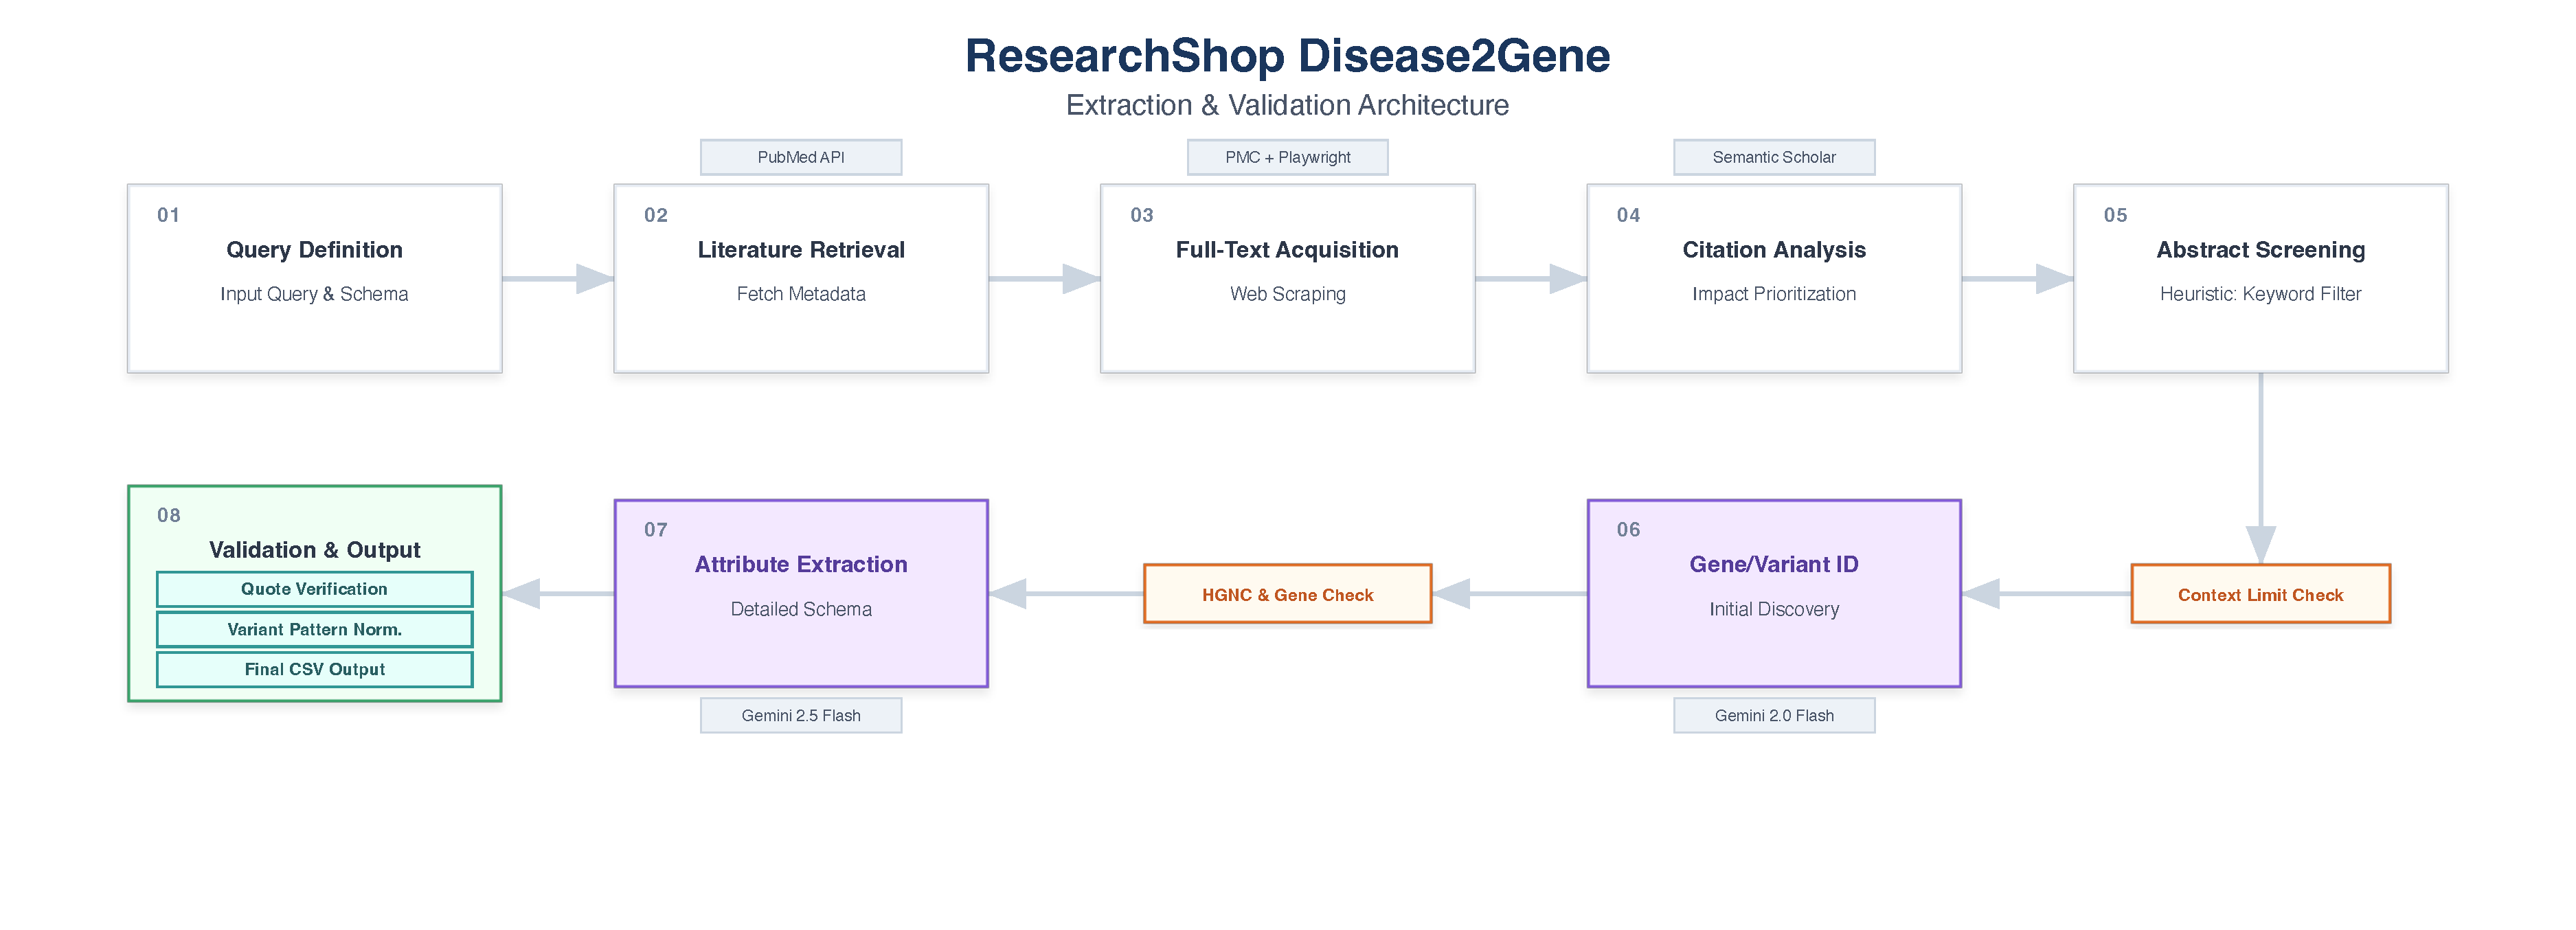
\includegraphics[width=0.95\textwidth]{architecture_diagram_en.pdf}
    \caption{ResearchShop pipeline architecture showing the eight processing stages. Rectangles represent processing stages; parallelograms indicate external API dependencies (PubMed, Semantic Scholar, Gemini LLMs). Stages 6--7 use Gemini LLMs for extraction; Stage 8 applies validation heuristics.}
    \label{fig:pipeline-architecture}
\end{figure*}

\subsection{Schema-Driven Extraction}
The system is designed for flexibility and scale. Users define a custom output schema as a JSON structure where each field represents a desired attribute with a natural language description:

\begin{lstlisting}[language=Python,basicstyle=\footnotesize\ttfamily,frame=single]
schema = {
  "gene_symbol": "Official HGNC gene symbol",
  "variant_hgvs": "Variant in HGVS nomenclature",
  "pathogenicity": "Clinical significance 
                    (pathogenic, benign, VUS)",
  "functional_impact": "Effect on protein function"
}
\end{lstlisting}

The pipeline dynamically prompts the LLM to extract these specific attributes. This enables researchers to customize extraction for different contexts (e.g., pharmacogenomics, rare diseases) without code modifications.

\subsection{Implementation Details}
\paragraph{Parallel Processing} Full-text extraction uses \texttt{ThreadPoolExecutor} with configurable workers (default: 3) and per-PMID timeouts (default: 120 seconds). AI analysis runs in separate processes using \texttt{multiprocessing} to achieve true parallelism and avoid GIL limitations.

\paragraph{Caching} Full-text content is cached using compressed pickle files (gzip, 60--80\% size reduction). Gene validation results use LRU cache (2000 entries) to prevent redundant API calls.

\paragraph{Error Handling} The pipeline implements retry logic with exponential backoff for transient failures, multiple timeout mechanisms, fallback strategies (PMC → Trafilatura → Playwright), and graceful degradation under rate limits.

\subsection{Desktop Application}
\label{subsec:desktop-app}
To enable non-technical users to run the pipeline locally, we provide a cross-platform desktop application with a graphical user interface (GUI). The application is built using CustomTkinter~\cite{customtkinter} and can be packaged as standalone executables (.exe for Windows, .app for macOS) using PyInstaller.

The GUI provides:
\begin{itemize}
    \item \textbf{API Configuration}: Input fields for Gemini API key, PubMed email, and optional PubMed API key.
    \item \textbf{Search Configuration}: PubMed query input with parameters for maximum papers and top-cited filtering.
    \item \textbf{Schema Editor}: JSON editor for defining custom output attributes.
    \item \textbf{Progress Tracking}: Real-time progress bar and log output during pipeline execution.
    \item \textbf{One-Click Export}: Direct access to output folder containing CSV results.
\end{itemize}

\paragraph{Installation} Users can either run the Python source directly (\texttt{python gui/disease2gene\_app.py}) or download pre-built executables from the GitHub releases page. The build script (\texttt{build\_app.py}) creates self-contained applications requiring no Python installation on the target machine.

\subsection{Validation Framework}
\label{subsec:validation}
A core contribution of this software is its robust defense against hallucinations. The validation framework operates at multiple levels, each targeting different types of potential errors (Figure~\ref{fig:validation-framework}).

\subsubsection{Gene Symbol Validation}
Every extracted gene is verified against authoritative databases using a two-tier strategy:

\begin{enumerate}
    \item \textbf{Local HGNC Database}: A cached copy of the HUGO Gene Nomenclature Committee database~\cite{bruford2023genenames} enables rapid lookups. The database includes official symbols, aliases, and previous symbols for comprehensive coverage.
    \item \textbf{API Fallback}: For queries not found locally, the system queries the HGNC REST API, then falls back to MyGene.info (human genes only) for additional coverage.
    \item \textbf{Fuzzy Matching}: When exact matches fail, the system queries MyGene.info to identify potential typos (e.g., ``BRAC1'' → ``BRCA1''), providing suggestions for manual review.
\end{enumerate}

This filters out non-existent or hallucinated gene symbols (e.g., ``BRCA3'', ``IL99'').

\subsubsection{Paper Text Verification}
The system performs exact-text searching to confirm that the valid gene symbol actually appears in the source paper text. This prevents ``contextual hallucinations'' where an LLM mentions a real gene from its training data that is not discussed in the paper. The algorithm uses word-boundary pattern matching:

\begin{lstlisting}[language=Python,basicstyle=\footnotesize\ttfamily,frame=single]
pattern = r'\b' + re.escape(gene) + r'(?![A-Za-z])'
gene_in_paper = bool(re.search(pattern, text.upper()))
\end{lstlisting}

The negative lookahead prevents false positives (e.g., ``CD4'' should not match ``CD40'').

\subsubsection{Filter Gate Architecture}
Gene Symbol Validation and Paper Text Verification form a combined \textbf{filter gate}: an association must pass \textit{both} checks to proceed. If either fails, the association is filtered out entirely. This dual requirement is critical for anti-hallucination, as it catches both:
\begin{itemize}
    \item Invalid symbols not in any database
    \item Valid symbols from LLM training data not in the source paper
\end{itemize}

\subsubsection{Variant Pattern Matching}
Extracted variants are validated against HGVS nomenclature patterns~\cite{den2016hgvs} to ensure structural correctness. Recognized patterns include:

\begin{itemize}
    \item Protein substitution: \texttt{p.Arg175His}
    \item Coding substitution: \texttt{c.1234A>G}
    \item Genomic substitution: \texttt{g.123456A>T}
    \item dbSNP identifiers: \texttt{rs123456}
    \item Simple amino acid notation: \texttt{R175H}
\end{itemize}

Both three-letter (Arg, His) and single-letter (R, H) amino acid codes are recognized. Generic descriptions (``mutation'', ``pathogenic variant'') are rejected as insufficiently specific.

\subsubsection{Quote Verification}
To combat fabricated evidence, the system extracts supporting quotes provided by the LLM and verifies their existence in the paper text. The verification process employs:

\begin{itemize}
    \item \textbf{Exact matching}: Normalized text comparison after lowercasing and whitespace normalization.
    \item \textbf{Fuzzy matching}: For citations with $\geq$5 words, if $\geq$80\% of significant words appear in the paper, the citation is considered valid.
\end{itemize}

Citation confidence scores are computed based on match type and length (longer citations = higher confidence). Results are stored as metadata for downstream filtering.

\subsubsection{Confidence Scoring}
The validation framework produces an overall confidence score:

\begin{equation}
C_{total} = C_g + C_v
\end{equation}

where $C_g = 0.7$ if the gene passes HGNC validation (or 1.0 for gene-only associations), and $C_v = 0.3$ if the variant passes pattern matching. Citation validation produces separate metadata and does not affect the core confidence calculation, enabling independent filtering on citation quality.

\section{Illustrative Examples}
\label{sec:examples}

\subsection{Evaluation Dataset}
We evaluated the software on a manually curated dataset of 19 full-text papers regarding Multisystem Inflammatory Syndrome in Children (MIS-C), a rare but severe condition following SARS-CoV-2 infection. The test corpus comprises peer-reviewed publications spanning multiple study types (WES, transcriptomics, GWAS, DNA methylation) from 2011--2023.

The ground truth includes 103 gene-disease associations across 103 unique genes, representing diverse immunological pathways relevant to MIS-C pathogenesis. All ground truth genes were verified to appear in their corresponding paper text before evaluation.

\subsection{Extraction Performance}
Table~\ref{tab:performance} presents aggregate extraction performance across five independent runs (to assess LLM reproducibility).

\begin{table}[htbp]
\centering
\caption{Extraction performance metrics (mean $\pm$ std, 5 runs)}
\label{tab:performance}
\begin{tabular}{@{}lr@{}}
\toprule
\textbf{Metric} & \textbf{Value} \\
\midrule
Papers Processed & 19/19 (100\%) \\
Full-Text Success & 19/19 (100\%) \\
Ground Truth Genes & 103 \\
\midrule
True Positives & 99.2 \\
False Negatives & 3.8 \\
\midrule
Recall & 0.963 $\pm$ 0.014 \\
Precision (standard) & 0.207 $\pm$ 0.013 \\
\textbf{Precision (GT-Adjusted)} & \textbf{0.978 $\pm$ 0.004} \\
\midrule
\textbf{Hallucination Rate} & \textbf{0.0\%} \\
\bottomrule
\end{tabular}
\end{table}

The pipeline achieved \textbf{96.3\% recall}, successfully identifying 99 of 103 ground truth genes. The standard precision of 0.207 reflects comprehensive extraction versus selective manual curation. However, the \textbf{GT-Adjusted Precision} of \textbf{0.978} more accurately reflects extraction quality: 99.5\% of ``false positives'' are valid genes appearing in paper text that curators chose not to annotate.

Most critically, the \textbf{hallucination rate was 0.0\%}---zero invalid gene symbols across all runs. This demonstrates the exceptional effectiveness of the multi-layer validation framework.

\subsection{Validation Ablation Study}
Table~\ref{tab:ablation} compares performance with and without validation heuristics.

\begin{table}[htbp]
\centering
\caption{Impact of validation heuristics (mean, 5 runs)}
\label{tab:ablation}
\begin{tabular}{@{}lccc@{}}
\toprule
\textbf{Configuration} & \textbf{Precision} & \textbf{Recall} & \textbf{F1} \\
\midrule
Validation Disabled & 0.173 & 0.973 & 0.293 \\
Validation Enabled & 0.207 & 0.963 & 0.341 \\
\midrule
\textbf{Change} & \textbf{+19.7\%} & \textbf{-1.0\%} & \textbf{+16.4\%} \\
\bottomrule
\end{tabular}
\end{table}

Enabling validation improved precision by 19.7\% with only a 1.0\% reduction in recall. The validation framework effectively filters noise while preserving legitimate findings.

\subsection{Comparison with PubTator Central}
We compared ResearchShop against PubTator Central~\cite{wei2019pubtator}, a widely-used biomedical NER system (Table~\ref{tab:pubtator}).

\begin{table}[htbp]
\centering
\caption{ResearchShop vs. PubTator Central}
\label{tab:pubtator}
\begin{tabular}{@{}lcc@{}}
\toprule
\textbf{Metric} & \textbf{ResearchShop} & \textbf{PubTator} \\
\midrule
Genes Extracted & 481 & 123 \\
GT Genes Found & 99/103 (96\%) & 63/103 (61\%) \\
\midrule
Recall & 0.963 & 0.612 \\
GT-Adjusted F1 & \textbf{0.971} & 0.733 \\
\bottomrule
\end{tabular}
\end{table}

ResearchShop demonstrated significantly higher recall (96.3\% vs 61.2\%). With GT-Adjusted metrics, ResearchShop achieves \textbf{F1 = 0.971} versus PubTator's 0.733. ResearchShop's full-text LLM-based extraction completely subsumes PubTator's coverage for this evaluation dataset.

\subsection{Error Analysis}
The 4 missed genes involved specialized nomenclature: \textit{DSEA} (non-standard), \textit{HLA-DP} (collective term), \textit{IGHV1-69} (immunoglobulin nomenclature), and \textit{CD4} (technical context). Zero false negatives were caused by the LLM failing to identify genes with standard nomenclature.

\subsection{Cost Analysis}
Processing 19 papers cost approximately \$1.85 USD (average \$0.10/paper). This represents a \textbf{99\% cost reduction} compared to manual curation (estimated 30--60 minutes per paper at \$50/hour expert rate).

\section{Impact}
\label{sec:impact}

\subsection{Democratizing Literature Mining}
ResearchShop Disease2Gene democratizes access to large-scale literature mining. By automating full-text acquisition and providing a validated extraction pipeline, it allows individual researchers to perform systematic reviews that would otherwise require teams of curators.

\subsection{Clinical and Research Applications}
\begin{itemize}
    \item \textbf{VUS Resolution}: Accelerates identification of evidence supporting variant classification by systematically mining published genetic associations.
    \item \textbf{Rare Disease Research}: Enables comprehensive literature surveys for conditions with limited, scattered publications.
    \item \textbf{Drug Target Discovery}: Supports identification of gene-disease associations relevant to therapeutic development.
    \item \textbf{Precision Medicine}: Provides evidence synthesis for personalized treatment recommendations.
\end{itemize}

\subsection{Scalability}
Based on observed performance (\$0.10/paper, 100\% completion rate), the system scales economically:

\begin{itemize}
    \item 100 papers: \$10 (vs. \$3,750 manual)
    \item 1,000 papers: \$97 (vs. \$37,500 manual)
    \item 10,000 papers: \$970 (vs. \$375,000 manual)
\end{itemize}

\subsection{Unique Contributions}
The software fills a critical gap:
\begin{itemize}
    \item \textbf{Full-text processing}: Unlike abstract-only tools, captures evidence from Results/Methods sections.
    \item \textbf{Validated extraction}: Multi-layer framework achieves 0\% hallucination rate.
    \item \textbf{Schema flexibility}: User-defined attributes without code changes.
    \item \textbf{Evidence traceability}: Mandatory citations enable human verification.
\end{itemize}

\section{Conclusions}
\label{sec:conclusions}
We have presented ResearchShop Disease2Gene, a validated pipeline for gene-disease association extraction from full-text biomedical literature. By integrating multi-strategy full-text acquisition with a multi-layer anti-hallucination framework (HGNC validation, paper text verification, variant pattern matching, quote verification), the software achieves 96.3\% recall with zero hallucinations and a GT-Adjusted F1-score of 0.971.

The pipeline completely subsumes the coverage of traditional NER approaches like PubTator Central while providing structured, schema-driven output with evidence traceability. At \$0.10 per paper, it offers a 99\% cost reduction compared to manual curation, enabling literature-scale systematic reviews.

\paragraph{Future Work} Planned enhancements include: (1) multi-modal extraction from figures and tables using vision-language models; (2) deeper integration with clinical databases (ClinVar, OMIM); (3) specialized handling of non-standard nomenclature (HLA, immunoglobulin genes); and (4) a web platform for non-technical users.

\section*{Acknowledgements}
We acknowledge the support of the Interdisciplinary Centre for Mathematical and Computational Modelling (ICM) at the University of Warsaw.

\bibliography{../../references}

\end{document}
